Ici vont être résumé les idées principales de \cite{Ganin15}.

\subsection{Rappel sur l'adaptation de domaine} % (fold)
\label{sub:rappel}

L'adaptation de domaine consiste à adapter un modèle entraîné sur certaines
données pour une utilisation sur des données similaires.
Ces nouvelles données sont suffisamment différentes pour endommager les 
performances du modèle. L'adaptation de domaine vise donc à réduire au mieux
cette perte de performance.

On sépare donc les domaines en un domaine Source $D_S$ et un ou plusieurs domaines 
Cibles $D_T$. On cherche à réduire le risque sur le/les domaine(s) Cible(s) $R_{D_T}$.

De plus on ne dispose pas de données annotées dans le domaine Cible. Il nous faut
nous contenter de celles du domaine Source. Cependant la tâche reste exactement la
même, seule la distribution change.

On a donc un seul problème mais les données sont 
tirées de diverses distributions plus ou moins différentes desquelles le modèle
doit extraire les informations pertinentes afin de résoudre le problème.

Selon \cite{BenDavid} le risque sur le domaine Cible est majoré par:
$$ R_{D_T} \le R_{D_S} + \mathcal{H}\text{-divergence}(S,T) + \beta + C $$

où $\beta$ est un terme lié à la capacité de la classe de modèle $\mathcal{H}$
à être efficace sur les deux distributions et $C$ est un terme principalement
lié à la VC-dimension et à la quantité de donnée disponnible.

C'est la $\mathcal{H}\text{-divergence}$ qui va nous intéresser ici.
Il s'agit d'une mesure de la distance entre le domaine Source et Cible.
$\mathcal{H}\text{-divergence}$ est la capacité du meilleur modèle 
$\eta^*\in\mathcal{H}$ à séparer les éléments du domaine Source $D_S$ et du
domaine Cible $D_T$. Autrement dit la capacité de $\eta^*$ à classifier les 
données selon leur origine.

On a donc deux problèmes distincts sur les même données. L'un est le problème que 
l'on cherche à résoudre, ie construire un modèle $h: x \in D^X \mapsto y \in D^Y$
qui trouvera les labels $y$ en fonction des données $x$.
L'autre problème $\eta: x \in D^X \mapsto y_D \in [0..n_{domain}]$ qui consiste
à trouver l'origine des données (quel domaine/distribution).
On souhaite construire un modèle qui rend efficace $h$ mais qui rend 
difficile $\eta$.

Puisque l'on cherche à réduire la $\mathcal{H}\text{-divergence}$ l'idée est 
de créer $\mathcal{H}$ "correctement".
Pour cela on va construire des réseaux de neurones incapables de déterminer
l'origine $y_D$ des exemples $x$.

% subsection rappel (end)
\subsection{Méthode proposée} % (fold)
\label{sub:methode}

On cherche donc à résoudre deux problèmes s'opposant l'un l'autre. D'une part
on souhaite améliorer au mieux le réseau pour qu'il soit efficace sur les
données d'entraînement. D'autre part on souhaite qu'il n'utilise que des 
descripteurs pertinent pour les deux distributions.

On cherche à rendre \emph{mauvais} le réseau sur la séparation des exemples
selon leur origine, ce qui revient à faire le contraire d'un classifieur. Et
à le rendre \emph{bon} sur la classification des exemples selon leur label.
On a donc deux classifications adverses en sortie du réseau.
Ainsi lors de la propagation arrière il est possible de propager un gradient
par tâche de classification. Puis lors de la mise à jour des paramètres 
exécuter une \emph{descente} de gradient pour la labellisation et une 
\emph{monté} de gradient pour la séparation des domaines.

L'objectif étant de construire une représentation commune pour les diverses 
distributions. En rendant le réseau "aveugle" sur l'origine des exemples
on le force à utiliser les informations communes aux différents domaines.
Cette représentation sera utilisée par la suite du réseau pour résoudre la
classification.
De cette façon on espère pouvoir optimiser le réseau à classifier les exemples
efficacement sur le domaine Cible.
Il est bien entendu nécessaire de régler le compromis entre les deux objectifs,
les deux gradients. Ceci introduit un nouvel hyper-paramètre $\lambda_{D}$.

Une astuce donnée par les auteurs sur l'implémentation d'un tel réseau dans 
les librairies déjà existante consiste à insérer une couche renversant le 
gradient lors de la propagation arrière provenant de la partie classifiant
les exemples selon leur origine et ne touchant pas au données lors 
de la propagation avant. L'architecture général est rappelée figure 
\ref{fig:arch}.

\begin{figure*}[htbp]
\centering
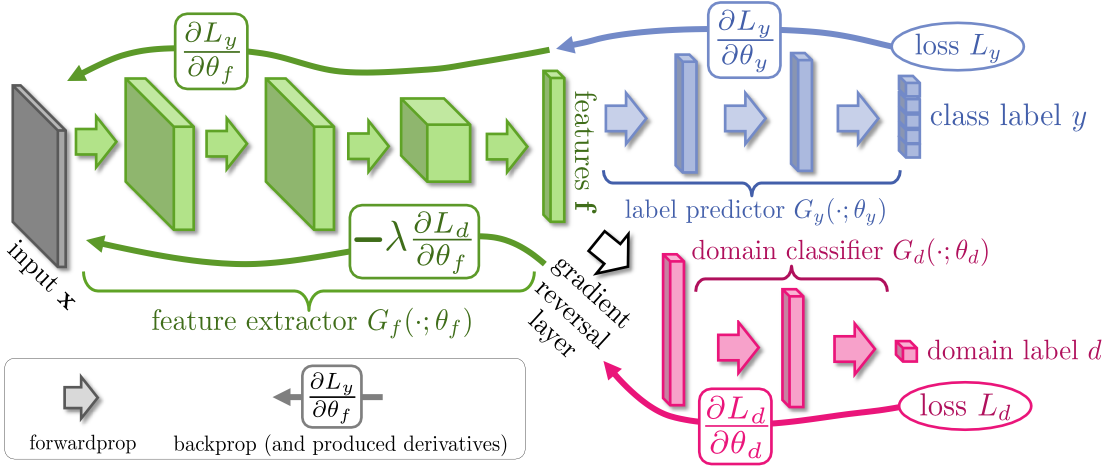
\includegraphics[width=\textwidth]{fig/arch.png}
\caption{Architecture des réseaux adversiaux}
\label{fig:arch}
\end{figure*}

Il reste maintenant à déterminer les hyper-paramètres de notre réseau : 
$\lambda_{D}$, l'architecture du réseau, le pas d'apprentissage, etc.

Puisque l'on ne dispose pas des labels pour les exemples issus du domaine Cible
Il faut trouver un autre moyen pour estimer les performances du modèle.

Ce problème a été abordé dans \cite{Zhong}. La solution proposée, \emph{validation 
inversée croisée} consiste à dire que :

Si le modèle $h$ est performant sur le domaine Cible alors les labels 
prédis sur les données Cibles sont justes. Il est alors possible de s'en servir
pour construire un modèle qui s'adapte dans l'autre sens (du domaine Cible 
vers le domaine Source) et prédire avec précision les labels du domaine Source
que l'on connaît. C'est donc les résultats de ce modèle 'renversé' $h_r$ qui 
indiqueront les performances des hyper-paramètres choisis. 

Tout comme dans le cas de la validation simple, cette méthode peut être 
exécutée sur des découpages différents de l'ensemble des données
afin d'obtenir une estimation plus fine des performances. 
On met de coté une petite partie des données puis on entraîne les deux modèles
($h,h_r$) sur la grande partie restante. Finalement l'évaluation 
s'effectue sur la partie mise de coté.

% subsection méthode (end)
